\documentclass{article}
\usepackage{graphicx} % Required for inserting images
\graphicspath{ {./images/} }
\usepackage[letterpaper,top=2cm,bottom=2cm,left=3cm,right=3cm,marginparwidth=1.75cm]{geometry}
\usepackage[square,numbers]{natbib}
\usepackage{makecell}

\bibliographystyle{abbrvnat}
\title{Unit 8 Learning Outcomes}
\author{Chris Hadden}
\date{}

\begin{document}


\maketitle


\section{D1 Assess the impact of digital marketing on an identified product}

We are going to assess some real life marketing campaigns and try to assess where they succeeded or where they failed.
As a part of this assessment we are going to determine
\begin{itemize}
\item What the goals of each campaign were
\item How the adverts were distributed
\item Who they were aiming the adverts at
\item And what their overall impression was
\end{itemize}

\begin{table}[h!]
    \centering
    \begin{tabular}{|p{0.3\textwidth}|p{0.6\textwidth}|}
       \hline
       \multicolumn{1}{c}{\bfseries Company Name} & \multicolumn{1}{c}{\bfseries What was positive about it?}  \\
             \hline
         John Lewis Christmas Campaigns & John Lewis' Christmas campaigns have become themselves a part of the UK's Christmas traditions. No other retailer has quite managed to get the same response as the John Lewis adverts. It has been stated that 81\% of consumers in the UK and Ireland think it is important for brands to raise awareness and take a stand on sensitive topics. Clearly this point of view has translated into social media traction for John Lewis \cite{JohnLewisChristmasCampaigns}


They have managed to recieve a huge 94\% postive sentiment and recently had the most anticipated advert since 2011. \cite{JohnLewisPowerful}  John Lewis have somehow managed to capture an emotional appeal with out coming over as soppy or sentimental. This is impressive as their main audience is family and particu- larly children where pulling on the heart strings would be too obivous. Possibly their secret weapon is an epic experience.  In thier 2019 advert they used fantasy which was aimed at adults but also worked for children. This got people talking and asking each other if they had seen it, which is makes it all the more memorable. \cite{JohnLewisPowerful} \\
        \hline
	This Girl Who Can Campaign & The Sport England advertising campaign, 'This Girl Can' was a surprise viral hit. It's aim was to appeal to all women and to inspire women to get fit and show how they can overcome any judgemental barrier they felt was in the way. Sport England invested heavilly in it, launching it on TV, social media and on posters. It shows women of all ages, shapes and races doing exercises and looking like they are sweaty and exhausted. It has proven to be inspirational to many women. \cite{ThisGirlCan}\\
        \hline
    \end{tabular}

\end{table}

\begin{table}[h!]
    \centering
    \begin{tabular}{|p{0.3\textwidth}|p{0.6\textwidth}|}
       \hline
       \multicolumn{1}{c}{\bfseries Company Name} & \multicolumn{1}{c}{\bfseries What was negative about it?}  \\
             \hline
	McDonalds & \#McDStories was a McDonalds campaign where they tried to demonstrate that McDonalds is a part of everyday American life. In general the advertising market thought that the concept was a very good one, they showed that the resteraunt is there in the good times and the bad. McDonalds showed images of their golden arches with signs underneath of everything from birthdays to funerals. Where it started to go wrong was when it made reference to major events such as 911. People felt that this was in poor taste. On top of that, on social media McDonalds had tried to start the hashtag \#McDStories, but "instead of nostalgic, fun memories, the campaign spurred a proliferation of jokes about obesity, horror stories from customers and complaints of poor treatment by ex-employees" and "the company had to remove the hash tag from Twitter due to the major negative reaction ... this didn’t stop consumers! They continued the conversation for over a week afterwards" as they personally had no control or regulation of the tag \cite{McD} \\
        \hline
	Dove & In 2017 Dove launched a campaign where women changing in to other women by removing thier shirts. While at first it looked like a stylishly edited attention grabbing advert, it was quickly spotted that what they had made was an advert that made it look like a black women revealed the inner white women inside her. 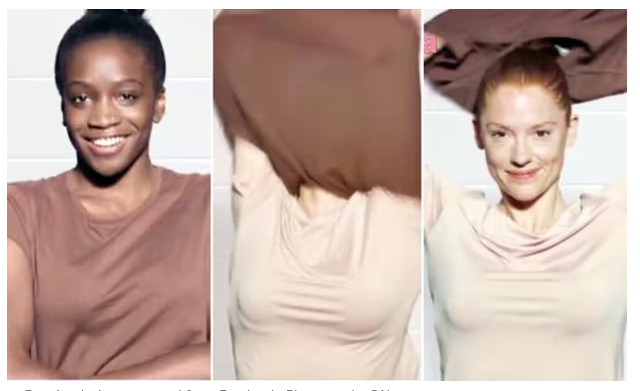
\includegraphics[scale=0.4]{Dove} \cite{Dove} This provoked an outcry, with women left wondering how a big company like Dove could make an advert that was so tone deaf. Dover had to remove the advert from Facebook and apologise. \\
        \hline
    \end{tabular}

\end{table}

For this task, you are required to create a written report on the impact of digital marketing on an identified
product. You will carry out research into a digital marketing campaign and the impact that the campaign had
on the identified product, assessing the impact whether it be positive, negative or a mixture of both.


o Then, you should go on to explain the digital marketing campaign you have researched, explaining
the following:
- What were the goals of the campaign?
- What channels were used?
- Who was the target audience?
- How much did it cost? (NB: don’t worry if you cannot find this information)
- What were the end results?
The following should be considered in your explanation:
- The role of marketing within business (Market research, raising awareness and affecting perception of
need via promotion and advertising, selling)
- Digital marketing as a business tool (Business establishment, business growth, business continuity)
- Strategies towards identified marketing goals (Identifying customers/markets, raising awareness,
increase sales, gaining information, gathering data and creating traffic)
o You will then need to assess the impact of the campaign – i.e. was the campaign successful or
not? You need to:
- Explain, in detail, what worked, what didn’t, feedback by the end user (where relevant),
what lessons could be/were learned.
o Conclusion/Summary


References:
These should be extensive! For images and any websites you have used for research, collect as you go, so
that you don’t have to go back and search for them later. Also, don’t forget to reference the Student
Textbook as well any other books/websites you have used during your research.
continued on next page...

\bibliography{bibliography}
\end{document}

         
